\chapter{Conceitos Básicos}
\label{sec:conceitos}

Esse capítulo revisa alguns conceitos básicos relacionados com jogos eletrônicos, tópico
principal deste TCC.

\section{Arquitetura de um jogo eletrônico multijogador com servidor central}
\label{sec:conceitos:servidores}
  Para quesito de comparação, é razoável termos em mente como se estrutura um jogo usual.
    
  \subsection{Separação do código}
    Um software cuja arquitetura de redes inclui um servidor central possui uma separação
    clara e bem definida de como um \textit{cliente} e um \textit{servidor} devem agir.
    
    \subsubsection{Software cliente}
      O software cliente é a parte que irá ser executada pelo público alvo do jogo, e é o que
      pode ser considerado como o "jogo em si". As escolhas de qual linguagem e/ou quais arcabouços
      utilizar, quais sistemas operacionais ou plataformas contemplar são todas realizadas em
      função do público alvo.
      
      Como jogos são interativos, essa parte sempre tem uma exigência de um ambiente gráfico,
      assim como uma placa de vídeo, na grande maioria das vezes com aceleração gráfica embutida em
      hardware.
      
    \subsubsection{Software servidor}
      O software servidor é visado em um público mais técnico, podendo até mesmo ser restrito dentro
      da empresa. O objetivo principal do servidor é permitir que diversos clientes consigam manter
      suas simulações do mundo do jogo em sincronia. Para tal, a sincronização pode ser desde apenas
      sincronizar entrada, como até mesmo ser o único responsável pela simulação, transformando os
      clientes em terminais burros.
      
      Em contraste com os clientes, as escolhas de linguagem, arcabouços, plataformas e outros são
      puramente econômicas, e não dependem das escolhas feitas para os clientes.
      
  \subsection{Integração}
    Tendo as duas partes separadas, elas não precisam ficar inteiramente separadas. As formas
    listadas a seguir são todas utilizadas por algum jogo comercial, com casos de mais de uma no
    mesmo jogo.
    
    \begin{enumerate}
      \item Acesso a um \textit{lobby} único, onde jogadores podem conversar um com os outros e
        procurar por partidas abertas e em andamento ou criar uma nova.
      \item Acesso a um serviço de \textit{matchmaking}, que encontra outros jogadores utilizando
        o mesmo serviço e cria uma partida para eles automaticamente.
      \item Acesso a uma lista de servidores dedicados cadastrados ao servidor central.
    \end{enumerate}
    
    Jogos recentes tendem a utilizar o item 2 exclusivamente, exemplos sendo \textit{Call of Duty:
    Modern Warfare 2\footnotemark{}} e \textit{Diablo III\footnotemark{}}, enquanto jogos antigos
    utilizavam as outras opções, como o item 1 em \textit{Diablo II\footnotemark{}} e o item 3 em
    \textit{Team Fortress 2\footnotemark{}}. Houve um claro avanço de preferir o item 2, com 
    \textit{Warcraft III\footnotemark{}} tendo o item 1 e 2, e uma atualização recente de 
    \textit{Team Fortress 2} introduziu o item 2.
    
    \addtocounter{footnote}{-5}

    \stepcounter{footnote}\footnotetext{
      Página da franquia: \url{http://www.callofduty.com/} (última visita em 01/12/2013).
    }
    \stepcounter{footnote}\footnotetext{
      Página oficial: \url{http://us.battle.net/d3/pt/} (última visita em 01/12/2013).
    }
    \stepcounter{footnote}\footnotetext{
      Página oficial: \url{http://us.blizzard.com/en-us/games/d2/} (última visita em 01/12/2013).
    }
    \stepcounter{footnote}\footnotetext{
      Página oficial: \url{http://www.teamfortress.com/} (última visita em 01/12/2013).
    }
    \stepcounter{footnote}\footnotetext{
      Página oficial: \url{http://us.blizzard.com/en-us/games/war3/} (última visita em 01/12/2013).
    }
    
  \subsection{Comunidade}
    Uma forma que algumas empresas usam para colaborar com a comunidade de um jogo é de, além de
    distribuir o cliente do jogo, distribuir um software para realizar exclusivamente a parte
    do servidor. Com acesso e esse software, chamado de \textit{servidor dedicado}, a comunidade
    pode por si só criar a manter servidores, que podem ser melhores que os oficiais para casos
    específicos. Exemplos de uso do servidor dedicado seria um servidor local para um torneio, 
    diminuindo a latência nas partidas, e removendo a dependência de uma conexão com a Internet.

\section{Redes Peer-to-peer}
\label{sec:conceitos:redes}

  \begin{figure}[h]
    \begin{centering}
    \fbox{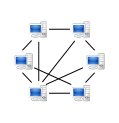
\includegraphics[width=0.45\textwidth]{../poster/p2p-network.png}}
    \fbox{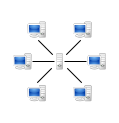
\includegraphics[width=0.45\textwidth]{../poster/server-based-network.png}}
    \caption{Comparação de rede Peer-to-peer (Esquerda) com Cliente-Servidor (Direita). \\
      Fonte: Baseado em figura de Wikimedia Commons (\url{http://commons.wikimedia.org/wiki/File:Computer_n_screen.svg}
      Última visita em 01/12/2013).
    }
    \end{centering}
  \end{figure}

  Uma rede peer-to-peer é um tipo de arquitetura de rede descentralizada e distribuída
  onde cada nó individual da rede atua como consumidor e fornecedor de recursos,
  simultaneamente, em contraste com redes cliente-servidor onde alguns nós apenas
  requisitam serviços fornecidos por servidores centrais. \cite{peertopeer:definition}
  
  Existem diversas formas para esses nós individuais, chamados de \textit{peers}, encontrarem
  recursos na rede e calcular rotas, em geral utilizando uma rede sobreposta (\textit{overlay
  network}) ao TCP/IP, permitindo que os peers se comuniquem diretamente um com os outros.
  
  Redes peer-to-peer podem ser classificadas de acordo com a organização da rede sobreposta:
  \begin{itemize}
    \item Redes Não-Estruturadas: Não existe nenhuma regra para a estrutura da rede, tornando impossível
        buscas eficientes, mas resistente a ataques.
    \item Redes Estruturadas: A rede sobreposta é organizada numa topologia específica, permitindo a busca
        eficiente por recursos específicos, mesmo aqueles raros. No entanto, implica num consumo maior de
        processamento e memória de todos os peers.
    \item Redes Híbridas: Uma combinação do modelo peer-to-peer com o cliente-servidor. Costuma incluir um
        servidor que auxilia os peers a encontrar outros peers.
  \end{itemize}
  
  Um exemplo famoso de uma rede peer-to-peer é o BitTorrent. Nela, um usuário utiliza um
  arquivo de meta-dados \textit{.torrent} para conhecer um servidor responsável pelo arquivos
  chamado \textit{tracker} e dados sobre os arquivos. O cliente se anuncia para o \textit{tracker} que
  por sua vez informa o cliente de outros peers que estão trabalhando com o mesmo \textit{.torrent}.
  Nesse caso, a rede pode ser considerada como híbrida.
  
  Uma extensão adicionada posteriormente ao BitTorrent é a tabela de hash distribuída (DHT).
  A DHT é uma forma de remover a necessidade dos \textit{trackers}, utilizando uma rede distribuída
  para encontrar os peers diretamente. Nesse caso, a rede pode ser considerada como estruturada.

\section{Vikings}
\label{sec:conceitos:vikings}
  O \textit{vikings}\footnotemark{} é um software livre produzido numa experiência de mini-projetos
  realizada pelo USPGameDev\footnotemark. Foi desenvolvido em Janeiro e Fevereiro de 2013 por
  Henrique Gemignani Passos Lima e Wilson Kazuo Mizutani utilizando a LÖVE, um arcabouço para jogos
  2D em Lua\footnotemark{}. A figura 2.2 apresenta uma \textit{screenshot} do vikings.
  
  \begin{figure}
    \label{sec:conceitos:vikings:screenshot}
    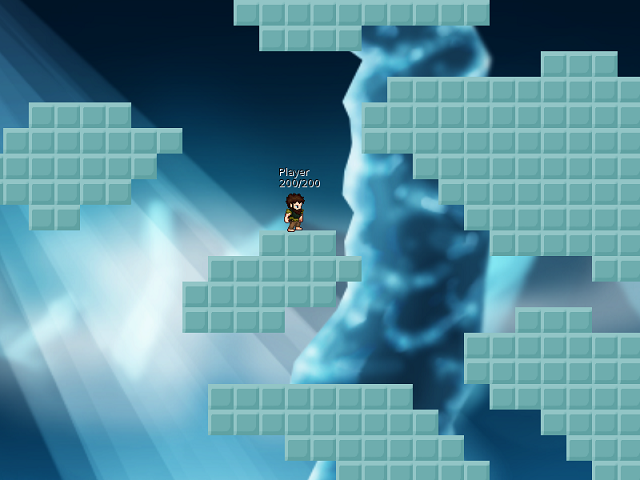
\includegraphics{imagens/vikings-1.png}
    \caption{Imagem do vikings}
  \end{figure}
  
  \addtocounter{footnote}{-3}

  \stepcounter{footnote}\footnotetext{
    Página do projeto: \url{http://uspgamedev.org/projetos/vikings/} (última visita em 23/11/2013).
  }
  \stepcounter{footnote}\footnotetext{
    O USPGameDev é um grupo de pesquisa e desenvolvimento de jogos da Universidade de São Paulo.
    Página oficial: \url{http://uspgamedev.org/} (última visita em 03/09/2013).
  }
  \stepcounter{footnote}\footnotetext{
    Página oficial: \url{http://www.lua.org/} (última visita em 23/11/2013).
  }

  \subsection{O Jogo}
    Em \textit{vikings}, você controla um jovem viking que sonha em se tornar o líder de sua vila. Para tal,
    você sai em busca de aventuras, buscando experiência, riquezas e equipamentos poderosos, para que um dia,
    você seja forte o suficiente para desafiar e derrotar o seu líder, tomando o seu lugar.
        
  \subsection{Jogabilidade}
    É um jogo de plataforma 2D com gráficos 2D, com mapas gerados procedimentalmente. Com o intuito de garantir
    que todo mapa gerado é possível, e numa tentativa de introduzir alguma profundidade e dificuldade, é
    possível dar quantas \textit{arrancadas} você quiser, mesmo estando no ar, e um único pulo no ar. No
    entanto, bater com a sua arma numa parede concede mais um pulo, permitindo ao jogador que ele escale
    paredes.
    
  \subsection{Detalhes Técnicos}
    Uma lista de conceitos e/ou algorítimos interessantes presentes no código:
    
    \subsubsection{Orientação a Objetos}
      Lua não possui orientação a objetos nativamente, mas utilizando as ferramentas da linguagem é possível
      implementar um sistema de orientação a objetos baseada em protótipos.
      No projeto, utilizamos o LUX\footnotemark{}, escrito pelo Wilson, em vez de repetir uma implementação.
      
      \footnotetext{
        Página do projeto: \url{https://github.com/Kazuo256/luxproject} (última visita em 23/11/2013).
      }
    
    \subsubsection{Geração procedimental de conteúdo}
      Para a geração dos mapas de cavernas, utilizamos o algoritmo de autômato celular, descrito no RogueBasin,
      \cite{roguebasin:cellularautomata} e levemente alterado para criar plataformas mais largas. Para
      evitar problemas de áreas desconexas, há um tratamento posterior do mapa onde áreas desconexas são unidas.
      Por fim, procuramos por plataformas vazias onde popular com monstros e itens.
